%!TEX root = ../template.tex
%%%%%%%%%%%%%%%%%%%%%%%%%%%%%%%%%%%%%%%%%%%%%%%%%%%%%%%%%%%%%%%%%%%
%% chapter1.tex
%% NOVA thesis document file
%%
%% Chapter with introduction
%%%%%%%%%%%%%%%%%%%%%%%%%%%%%%%%%%%%%%%%%%%%%%%%%%%%%%%%%%%%%%%%%%%

\typeout{NT FILE chapter1.tex}%

\chapter{Introduction}
\label{cha:introduction}

%INTRO
Collision avoidance is a crucial factor that permeates our society, and when it comes to automation, robots should aim for safety. However the baseline framework of the usual online safety critical control techniques could have some limitations. In the context of space, the high budget missions along with the limited size to carry resources like fuel..., the recurrent spacecrafts maneuvers to avoid collisions with debris \cite{hall2014history} (and other hazards), lead essentially to a need for safety and reliability, but welcome to improved performance and possible costs reductions.  

Previously, one of the most used collision avoidance control techniques used to be \glsxtrfull{APF} \cite{krogh1984generalized, khatib1986real}, analogous to an energy and its gradient to a guiding force. A technique not that robust, subject to relatively highly sensible performance according to the environment and with high necessity to a fine tuning of its parameters. 

Meanwhile, it arises in popularity the \glsxtrfull{CBF} that allows to design a controller aiming to online, keep a system safe \cite{ames2019control}. It is characterized by a control affine constraint that, if respected, contributes to forward invariance of a well defined safe set. Compared to the \glsxtrshort{APF}, the \glsxtrfull{CBF} reveal more appetence, it generates smoother trajectories and is able to deal with more complex scenarios \cite{singletary2021comparative}.

The \glsxtrshort{CBF} is a generalization of the \glsxtrfull{CLF} \cite{sontag1983lyapunov, ames2014rapidly}, however during problems generally used as keep away behaviour from the unsafe states whilst \glsxtrshort{CLF} imposing an approximation to an equilibrium point, i.e, inducing asymptotically stability to an desired equilibrium state. 

Initially the \glsxtrshort{CBF} proposed in \cite{ames2014control} were unbounded near the boundary being propitious to numerical problems. Beyond that, there it was proposed a \glsxtrfull{QP} formulation, combining the \glsxtrshort{CLF} and \glsxtrshort{CBF} in order to synthesize a controller that could achieve safety and stability of the system, which is not always possible.  Afterwards, \cite{xu2015robustness} presented the zeroing \glsxtrfull{CBF} solving previous problem, taking null values at the boundary of the safe set and establishing it as the standard. Regarding the \glsxtrshort{QP}, more recently \cite{ames2019control} proposed a solution to ensure feasibility, by softening the stability objective, but potentially leading to deadlock situations. More than that, in the given formulation, the \glsxtrshort{CLF-CBF} parameters are generally static, tuned according to a given problem, showing a decrease in performance as the scenario differs from what was initially conceptualized. The \glsxtrshort{QP} also lacks a prediction horizon, so the decision algorithm, in particular the \glsxtrshort{CBF}, just provides safety on the given instant, possibly resulting in states close to the boundary which demands returning high control inputs to maintain the system safe.

%APRESENTAÇÃO
The proposed techniques are compromised to deal with the respective characteristics. Among them the lack of adaptiveness through an offline (or at least opportunistic) optimization of the severity of the \glsxtrshort{CBF} condition, making use of algorithms  such as gradient descent \cite{ruder2016overview}, highly used in deep learning \cite{tian2023recent}, or a binary search \cite{lin2019binary} variation. There have been  Beyond that, it is proposed a way to deal with undesired (asymptotically stable) equilibria in the closed-loop system, by changing the stabilization objective from the \glsxtrshort{CLF}, forcing the convergence of the closed-loop system to a transitive deduced point on the boundary of the safe set, but essentially aiming to optimize the path taken, relative to the nominal \glsxtrshort{CLF-CBF} framework, avoiding the unwanted large inputs near the unsafe set while keeping the nominal speed of convergence. If it is not capable of reaching the desired state, through a \glsxtrshort{MPC}, sending the simulated trajectory as initial guess for a warm start optimization it is possible to mitigate the chances of a deadlock situation. 

%This work, aims to generalize the the given algorithms to high-order systems, as robotic systems such as spacecrafts are generelly governed by high relative-degree constraints, therefore \cite{ames2019control} came with \glsxtrfull{ECBF} as a solution to it while \cite{taylor2022safe} with backstepping which was the chosen one to apply on this thesis experiments.

%Relevant to say, \glsxtrshort{CBF} have been gaining lots of focus in reasearch, including in spacecrafts and satellites \cite{breeden2022predictive, breeden2021guaranteed}, \glsxtrfull{UAV} \cite{matias2025hybrid, singletary2021comparative}, among many others robotic systems \cite{ames2019control} (bipedal robots, multi-robot systems...). 

%EXTRAS
A \glsxtrshort{MPC} performs an optimization of multiple variables along an constrained receeding horizon (\glsxtrshort{MPC} applied in spacrafts rendezvous \cite{hartley2015tutorial, kaczmarek2023autonomous}), able to the incorporate \glsxtrshort{CBF} conditions to enforce safety of the close-loop system  \cite{grandia2021multi}, whilst \glsxtrshort{CLF-CBF} simply returns a single control input based on the given instant providing  faster computations.
The aim of this thesis is develop a low-effort \glsxtrshort{CLF-CBF} based decision algorithm, suited to spacecrafts (processors), that similar to \cite{matias2025hybrid, reis2020control} comes by founding a closed-form solution of the constrained \glsxtrshort{QP}. The given solution is periodic but potentially being approximately continuous with the implementation of circuits designed to process gradient descent methods or even the closed-form solution of the respective \glsxtrshort{QP} \cite{hao2025analysis}.

% Previous articles purpose variations of the technique which lack adaptiveness as their parameters are constant and tuned according to a particular problem need/experiment. The proposed algorithms present an offline (or at least opportunistic) optimization of the severity of the \glsxtrshort{CBF} condition, making use of algorithms  such as gradient descent \cite{ruder2016overview}, highly used in deep learning \cite{tian2023recent}, or binary search \cite{lin2019binary}.  

%The techniques presented here are designed to be able to deal with unsafe sets graphically with different shapes and sizes, usually delimited by an ellipsoide but like \cite{matias2025hybrid}, is given the \glsxtrshort{CBF} formulation that enables encoding the obstacles complex shapes by doing the polytope fit shown in \cite{molnar2023composing}.   
% Like \cite{reis2020control, matias2025hybrid}, it is proposed a way to deal with undesired (asymptotically stable) equilibria in the closed-loop system, by changing the stabilization objective from the \glsxtrshort{CLF}, forcing the convergence of the closed-loop system to a point on the boundary of the safe set, but essentially aiming to optimize the path taken, relative to the nominal \glsxtrshort{CLF-CBF} framework. If is not capable to reach the desired state, through a \glsxtrshort{MPC}, sending the simulated trajectory as initial guess for a warm start optimization it is possible to mitigate the chances of a deadlock situation.
This work aims to generalize the given algorithms to be able to deal with unsafe sets, usually delimited by an ellipsoide. Given the \glsxtrshort{CBF} formulation that enables encoding the obstacles complex shapes. \cite{molnar2023composing} presented a way to merge \glsxtrshort{CBF} via logical operations, providing a smooth approximation of the max and min functions representative of the AND OR operations.  

The proposed techniques , also extends to high-order systems, as robotic systems such as spacecrafts are generally governed by high relative-degree constraints, therefore \cite{ames2019control} came with \glsxtrfull{ECBF} as a solution to it while \cite{taylor2022safe} adapted to context of \glsxtrshort{CBF} backstepping~\cite{sepulchre2012constructive} which was the chosen one to apply on this thesis experiments.
Relevant to say, \glsxtrshort{CBF} have been gaining lots of focus in reasearch, including in spacecrafts and satellites \cite{breeden2022predictive, breeden2021guaranteed}, \glsxtrfull{UAV} \cite{singletary2021comparative}, among many others robotic systems \cite{ames2019control} (bipedal robots, multi-robot systems...). 

%OUTROS
Works in the area, such as \cite{reis2020control}, showed that the \glsxtrshort{QP} \cite{ames2019control} introduce undesired equilibrium points in the obstacles boundary and conditions that is propitious to happen. There have been ways proposed to address the problem \cite{braun2020comment, cortez2022compatibility}, between them, the \cite{reis2020control} presented a method as a way to deal with that, by composing a rotative \glsxtrshort{CLF} and adding to the \glsxtrshort{QP} formulation a \glsxtrshort{CBF} condition preventing the system convergence to the unwanted stabilization conditions related with the used \glsxtrshort{CLF}. Although the results don't show boundary equilibria, due to probably the \glsxtrshort{CLF} level set initial setup relative to the starting point the trajectories reveal undesired behaviours.

Meanwhile, \cite{matias2025hybrid} presents a collision avoidance hybrid \glsxtrshort{CLF-CBF} framework given a polytopic delimitation of the unsafe states. Its method proposes as a solution a switching mechanism between active half-spaces and associated (intermediate) equilibrium points able to converge to the desired equilibrium point.

Following a receeding horizon approach (like \glsxtrshort{MPC}), \cite{breeden2022predictive} formulates a \glsxtrshort{CBF} that under collision of a given nominal trajectory along the respective horizon, based on the supposing time until the next predicted collision and next local maximum of the \glsxtrshort{CBF} function is able to return a single control input preventing possible future collisions with minimal intrusion of the nominal controller.  

The proposed control techniques stand out by the fast computational speed, adaptatively capacity, options given the different scenarios and easy implementation. 

%ESTRUTURA
This thesis starts in chapter \ref{cha:methodology} with the section \ref{sec:clf_cbf} by introducing the methodology of the \glsxtrshort{CLF-CBF}, including the formulation for backstepping, for the polytope fit and the closed-form controller governed by those concepts. Secondly, it is presented the particular methods used by the proposed techniques, the different single parameter optimization algorithms \ref{sec:Single_Parameter_Optmization}, such as variations of gradient descent and the binary search method, and coming after, is shown how to obtain the obstacle contour point \ref{sec:Constraint_Contour_Point}. Given the presented contents, in section \ref{sec:Proposed_Decision_Algorithms} it's elaborated the proposed algorithms. Finally, in chapter \ref{cha:results} there are simulations of the developed algorithms in collision scenarios, applied on a mixed-relative-degree-two unicycle system and on a second-order perturbed orbital model, both with their \glsxtrshort{CLF} and \glsxtrshort{CBF} defined accordingly. In the results it is provided the computational time of the respective algorithms and also some performance data. Concluding with chapter \ref{cha:conclusion}, providing some reflections on this thesis results and some suggestions on how to continue this work.































%Excertos de coisas que estavam no template versão original



%\prependtographicspath{{Chapters/Figures/Covers/}}

% epigraph configuration
%\epigraphfontsize{\small\itshape}
%\setlength\epigraphwidth{12.5cm}
%\setlength\epigraphrule{0pt}

%
\includegraphics[width=0.1\linewidth]{NOVAthesisFiles/Images/novathesis-insignia}\hfill
%
\includegraphics[width=0.875\linewidth]{NOVAthesisFiles/Images/novathesis-text}

% \noindent This is the \gls{novathesis} \LaTeX\ template \ntindex[Template!]{Version} \novathesisversion\ from   {Template!date}\novathesisdate.

% \epigraph{
%   This work is licensed under the \href{https://www.latex-project.org/lppl/lppl-1-3c/}{\LaTeX\ Project Public License v1.3c}.
%   To view a copy of this \ntindex[Template!]{license}, visit the \href{https://www.latex-project.org/lppl/}{LaTeX project public license}.
% }

% \section{Welcome to the \novathesis\ Template}
% \label{sec:if_you_use_this_template}

%~\ref{cha:users_manual}.

% \subsection{Your Time is Precious}
% \label{sub:time_is_money}

%\emph{learning the rules} 

%\begin{tcolorbox}[colback=green!8]
%\\\parbox{\linewidth}{\raggedleft---~\emph{João Lourenço}}
%\end{tcolorbox}

%\href{https://www.paypal.com/donate/?hosted_button_id=8WA8FRVMB78W8}{\fcolorbox{DarkGreen}{gray!15}{\textbf{~HERE~}}} 


% \begin{figure}[htbp]
%     \centering
%     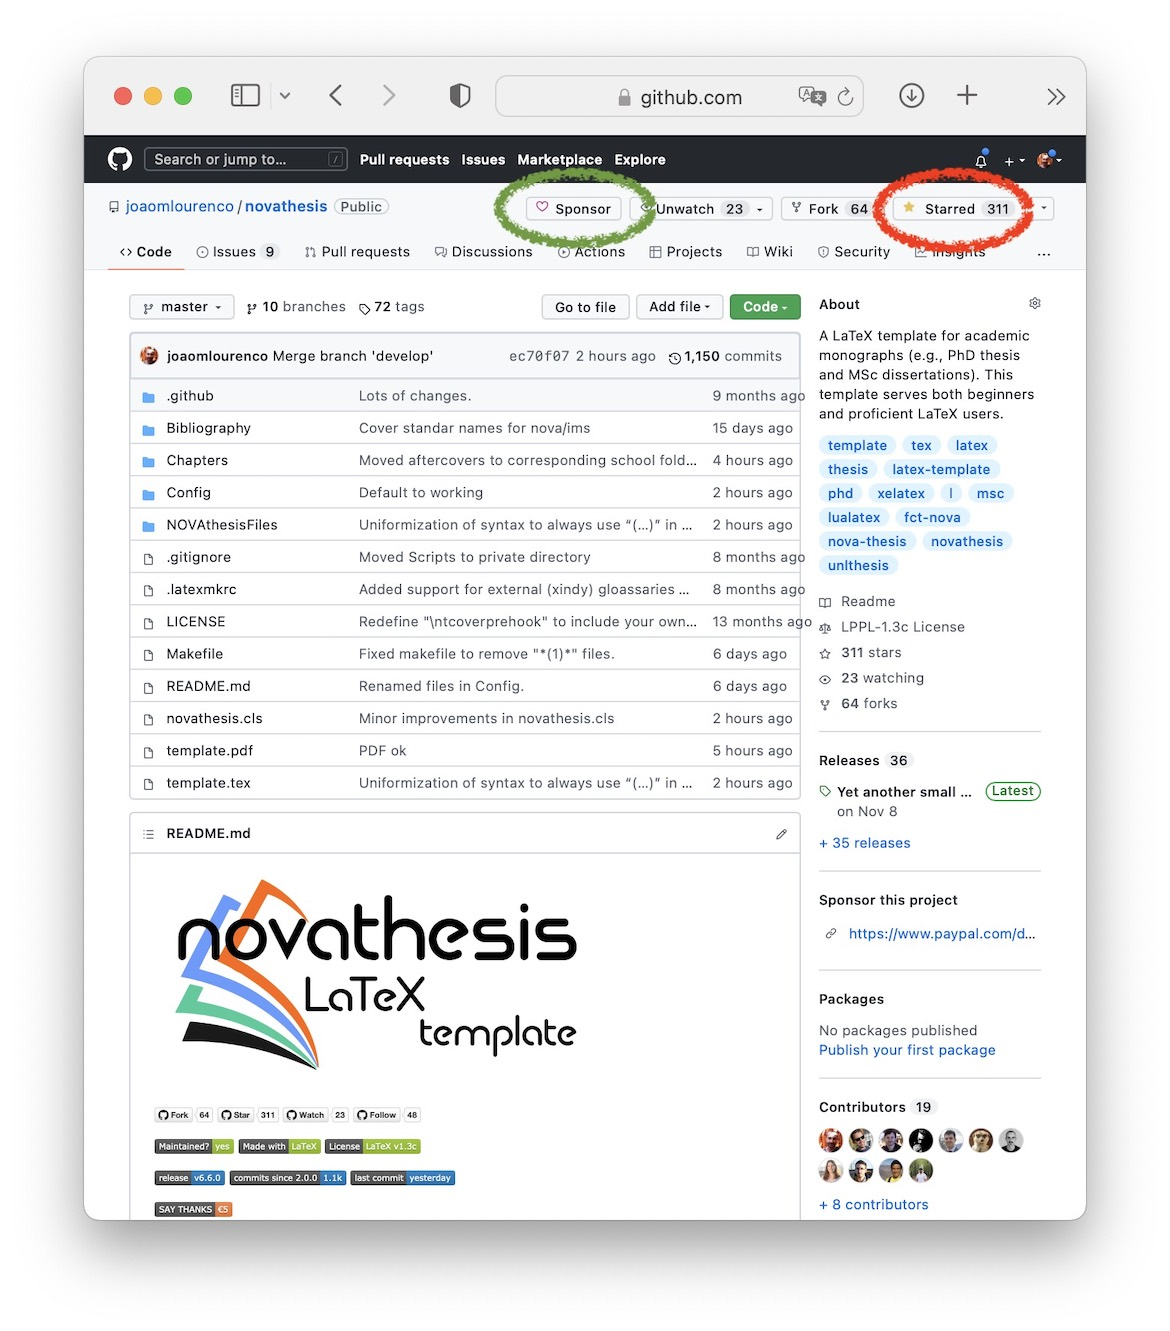
\includegraphics[width=0.5\linewidth]{github1}
%     \caption{The \gls{novathesis} project web page in GitHub.}
%     \label{fig:github}
% \end{figure}

% \section{The \emph{NOVAthesis} Template}
% \label{sec:a_bit_of_history}

% \ntindex[Template]{}

% \newenvironment{ntUniversity}[1]{
%   \renewcommand\tabularxcolumn[1]{m{##1}}% for vertical centering text in X column
%   % \renewcommand\cellgape{\Gape[1cm]}
%   % \setcellgapes{20pt}
%   % \makegapedcells
%   % % \setlength{\extrarowheight}{20pt}
%   % \renewcommand{\arraystretch}{2}
%   \rowcolors{1}{}{GhostWhite}
%     \xltabular{\linewidth}{cX}%
%       \caption{#1's Schools supported by the \gls{novathesis} template\label{tab:supported_schools_#1}}\\
%     \toprule%
%     \rowcolor{Gainsboro}%
%     & \Gape[1.5ex]{\thead[l]{#1}}\\
%     \midrule%
% }{%
%     \bottomrule
%     \endxltabular%
% }

% \makeatletter
% \newtoggle{coverspace}
% \newcommand{\docCover}[1]{%
%   \setlength{\fboxsep}{0pt}%
%   \togglefalse{coverspace}%
%     \Gape[1.5ex]{\begin{mcellbox}[cc]
%     \@for\myi:=#1\do{%
%       \fbox{\colorbox{White}{\includegraphics[align=c,width=1.5cm]{1up/\myi}}}%
%         \ifx\@xfor@nextelement\@nnil
%           % last iteration
%         \else
%           % not last iteration
%           \iftoggle{coverspace}{\togglefalse{coverspace}\\\\[-14pt]}{\toggletrue{coverspace}~}%
%         \fi
%   }%
%     \end{mcellbox}}
% }
% \makeatother
% \newcommand{\schlName}[3]{\textbf{#1} (\href{#3}{#2})}
% \newcommand{\degreeName}[3]{\newline\null\quad • #1 \href{#3}{(#2)}}

% \begin{ntUniversity}{NOVA University Lisbon}
%   {
%       \docCover{nova-fct-phd-en,nova-fct-msc-en}
%   } &  {
%     \schlName{NOVA School of Science and Technology}{FCT-NOVA}{https://www.fct.unl.pt}
%     \degreeName{All PhD Programs}{PhD}{https://www.fct.unl.pt/en/education/phd-programmes}
%     \degreeName{All MSc Programs}{MSc}{https://www.fct.unl.pt/en/education/master-degrees}
%   }\\
%   
% \end{ntUniversity}

% \newdata*{schlname}
% \newdata*{schlurl}
% \schlname(ea):={School of Architecture}
% \schlurl(ea):={https://www.uminho.pt/EN/uminho/Units/schools-and-institutes/Pages/School-of-Architecture.aspx}
% \schlname(ec):={School of Sciences}
% \schlurl(ec):={https://www.uminho.pt/EN/uminho/Units/schools-and-institutes/Pages/school-of-sciences.aspx}



% \subsection{Using Overleaf}
% \label{sub:using_overleaf}

% \ntindex[Installation!Overleaf]{}
% \ntindex[Using!Overleaf]{}

% \newcommand{\Overleaf}{\href{https://www.overleaf.com?r=f5160636&rm=d&rs=b}{Overleaf}}

% \begin{wrapfigure}{r}{0.3\linewidth}
% % \vspace*{-10ex}
% 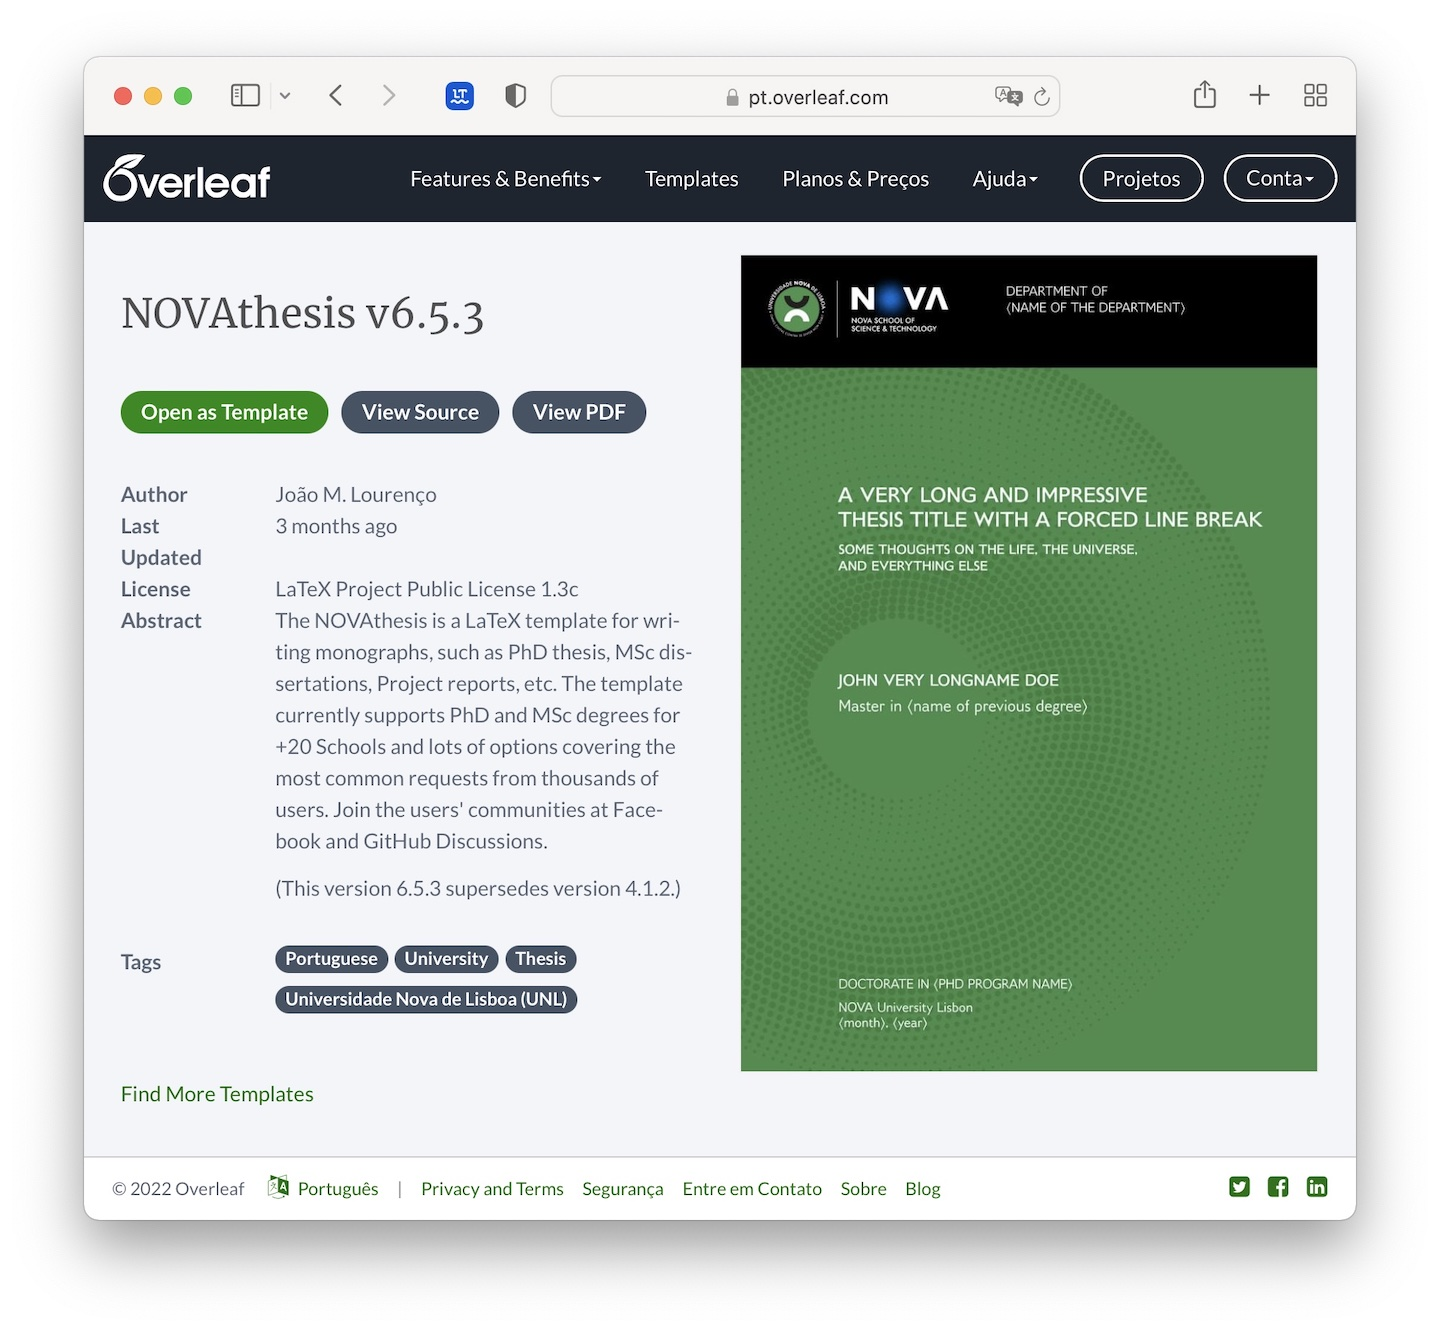
\includegraphics[width=\linewidth]{overleaf}%
% \caption{NOVAthesis template in Overleaf.}
% \label{fig:overleaf}
% \end{wrapfigure}
% \mbox{}\Overleaf\ is a collaborative cloud-based LaTeX editor used for writing, editing and publishing scientific documents. Like “Google Docs”,  

% \begin{tcolorbox}[colback=red!8]
% 	Notice that you need a (student) subscription to compile the \novathesis\ template in Overleaf, otherwise your compilation will always time out.
% \end{tcolorbox}

% \begin{description}
%   \item[Help:] If you just need some help, see above \Autoref{sec:getting_help}.
%   \item[Suggestion:] \ntindex[Suggestions]{} Do you have a suggestion/recommendation? Please add it to the wiki and help other users!
%   \item[Bug:] \ntindex[Bugs]{} Did you find a bug? Please open an issue. Thanks!
%   \item[New Feature:] \ntindex[Feature Requests]{} Would you like to request a new feature (or support of a new School)? Please open an issue. Thanks!

% \end{description}
